% ============================================================
%  第五章
% ============================================================
\section{单极子、Bogomolny 方程与 Atiyah--Hitchin 流形}
\markboth{第五章\ 单极子、Bogomolny 方程与 Atiyah--Hitchin 流形}{第五章\ 单极子、Bogomolny 方程与 Atiyah--Hitchin 流形}

\noindent{\small\color{shuyiGray}对应底本：原 p.25--p.28。}\par\medskip

\subsection{奇点：描述不完备之处}

\srcp{25}狄拉克曾考虑过 $U(1)$ 规范理论中的单极子，而在那个描述里，单极子是一个奇点。

\begin{figure}[htbp]
\centering
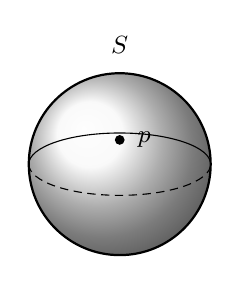
\begin{tikzpicture}[scale=1.1]
  \shade[ball color=gray!6] (0,0) circle (1.05);
  \draw[thick] (0,0) circle (1.05);
  \draw[densely dashed] (-1.05,0) arc (180:360:1.05 and 0.36);
  \draw (-1.05,0) arc (180:0:1.05 and 0.36);
  \fill (0.0,0.28) circle (1.6pt);
  \node[right=3pt] at (0.0,0.28) {\small $p$};
  \node[above] at (0,1.16) {\small $S$};
\end{tikzpicture}
\caption{狄拉克的描述里，单极子是空间中的一个奇点。场的方程在 $p$ 处失去意义，读者若只在这个层次上看，就会以为单极子“不是场”。}
\label{fig:singularity}
\end{figure}

我们所知道的物理方程并不完备；通常，一个物理问题的某种描述里的“奇点”，实际上是空间或时空中这样一块区域：在那里，给定的描述层次失效了，需要更完备的描述。比如说，电磁学在经典上——甚至在量子电动力学里——被描述为 $U(1)$ 规范理论；但在标准模型里，事实证明更完备的描述要求规范群是 $U(2)$——并带一个“希格斯机制”，用它来解释为什么这个理论对许多目的而言可以近似地当作 $U(1)$ 规范理论。

\subsection{\texorpdfstring{'t Hooft--Polyakov}{'t Hooft-Polyakov} 单极子：把奇点抹平}

\srcp{26}1970 年代初，'t Hooft 与 A.~M.~Polyakov 证明了：如果把 $U(1)$ 规范理论换成一个带“希格斯化”到 $U(1)$ 的 $SU(2)$ 规范理论——意思是，在低能观测中规范群被有效地约化到 $U(1)$——那么单极子就可以有一个完全光滑的描述。在这个描述里（而且是在 $e$ 很小的时候！），单极子对应于一个非线性偏微分方程的解。

\subsection{Bogomolny 方程}

\srcp{27}描述单极子的最简单的方程是“Bogomolny 方程”（由 E.~B.~Bogomolny 引入）：它是关于 $G$-丛 $E\to\RR^3$ 上的联络 $A$、以及取值于伴随丛 $\operatorname{ad}(E)$ 的零形式 $\phi$（“希格斯场”）的方程。方程是
\begin{equation}
  F=\star\,\dd_A\phi .
  \label{eq:bogomolny}
\end{equation}
这个方程算是四维瞬子方程在三维的某种表亲。它有许多迷人的性质，其中许多是 Atiyah 与 Hitchin 在他们 1988 年的书《磁单极子的几何与动力学》里探讨过的。除其他事情之外：Bogomolny 方程解的模空间是\emph{超 Kähler} 流形。对磁荷 $2$，那个“约化”模空间（把平凡的对称性约化掉）是四维的，Atiyah 与 Hitchin 显式地描述了它。这就是 Atiyah--Hitchin 流形：一个四维超 Kähler 流形，带 $SO(3)$ 对称性。

\subsection{同一时期的 Donaldson 理论}

\srcp{28}同一时期的另一项发展，也受到 Atiyah 的影响，是用非阿贝尔规范理论的瞬子构造出来的光滑四维流形的 Donaldson 理论。Atiyah 建议把 Donaldson 理论当作一个物理学家的问题来理解。到 1988 年，事情已经清楚：Donaldson 理论可以被理解为 $\cN=2$ 超杨--米尔斯理论的“扭曲版本”。要记得，$\cN=2$ 超杨--米尔斯理论几乎就是可能有 Montonen--Olive 对偶的理论的候选者：它满足 Olive 和我的判据，但不满足 Osborn 那个更精细的判据。$\cN=2$ 超杨--米尔斯理论与 Donaldson 理论的关系，提出了一个问题：在 $\cN=2$ 理论上的进展，会不会带来四维流形上的进展？不过，对此我是悲观的。

\begin{pizhu}{从奇点到孤子：Bogomolny 方程的能量下界}
设 $E\to\RR^3$ 是 $G$-丛，$A$ 是联络，$\phi\in\Gamma(\operatorname{ad}E)$ 是希格斯场，且 $|\phi|\to v$（$v$ 为真空期望值）当 $|x|\to\infty$。能量泛函是
\[
  E(A,\phi)=\int_{\RR^3}\Bigl(|F|^2+|D_A\phi|^2\Bigr)\dd^3x .
\]
把它配方：
\[
  E=\int|F-\star D_A\phi|^2\dd^3x+2\int F\wedge D_A\phi ,
\]
而第二项是全导数，等于 $\displaystyle 2\oint_{S^2_\infty}\phi\, F$。代入无穷远处的行为与大 $r$ 的 $F$，得
\[
  E\ \ge\ 4\pi v\,|m| ,
\]
其中 $m$ 是磁荷（第一陈数）。等号成立当且仅当 $F=\star D_A\phi$——这就是 Bogomolny 方程，而取等号的解叫 BPS 解。

两个推论。其一，这个下界对任意解都成立，所以它是“拓扑的”：只依赖 $m$ 与 $v$，不依赖耦合常数。其二，BPS 解满足一阶方程而不是二阶的 Yang--Mills--Higgs 方程，因此数学上更好处理：模空间的线性化方程是椭圆的一阶系统，而不是二阶的。Atiyah--Hitchin 的全部工作，都建立在这个“一阶化”之上。
\end{pizhu}

\begin{pizhu}{$SU(2)$ 磁荷 1 的显式解：Prasad--Sommerfield}
在 $SU(2)$ 情形，Bogomolny 方程有一个球对称的解析解。把李代数值写成 $\phi=\phi^a\sigma^a/2$、$A_i=A_i^a\sigma^a/2$，取
\[
  \phi^a=\frac{x^a}{r^2}\bigl(vr\coth(vr)-1\bigr),\qquad
  A_i^a=\varepsilon_{aij}\frac{x^j}{r^2}\Bigl(1-\frac{vr}{\sinh(vr)}\Bigr),
\]
就得到磁荷 $1$、能量恰为 $4\pi v$ 的解（Prasad--Sommerfield，1975；Bogomolny 同年给出）。它在 $r\to\infty$ 处趋于纯规范，在 $r\to0$ 处光滑——这正是第 25 页所说的“把奇点抹平”：不是把奇点藏起来，而是用一个处处正则的场论对象替代它。它在 $r\to\infty$ 处趋于纯规范，在 $r\to0$ 处光滑——这正是第 25 页所说的“把奇点抹平”：不是把奇点藏起来，而是用一个处处正则的场论对象替代它。
\end{pizhu}

\begin{pizhu}{为什么单极子模空间是超 Kähler}
把 $\RR^3$ 上的三个坐标方向看成三个复结构的方向，Bogomolny 方程 $F=\star D_A\phi$ 可以拆成三个实方程。用四元数的语言，它们分别是三个复结构 $I,J,K$ 下的“全纯性”条件，各对应一个矩映射。于是解的模空间是超 Kähler 商
\[
  \cM=\mu^{-1}(0,0,0)/\cG ,
\]
其中 $\cG$ 是规范群。Hitchin 在 1980 年代把这套构造系统化，并证明模空间上有三个相容的复结构。

“超 Kähler”意味着：模空间上有三个复结构 $I,J,K$，满足四元数关系 $I^2=J^2=K^2=IJK=-1$。这个结构是 Atiyah--Hitchin 分析单极子动力学的基础——他们把这套结构用在两单极子的情形，算出了完整的度量。
\end{pizhu}

\begin{pizhu}{Atiyah--Hitchin 流形与“第二单极子”}
磁荷 $2$ 的约化模空间是四维的，Atiyah 与 Hitchin 在 1985 年的两篇论文和 1988 年的书里给了它显式的度量。这个流形现在就叫 Atiyah--Hitchin 流形，记作 $\cM_2$。它的结构可以这样记：

\begin{itemize}
  \item 它是完备、非紧的四维超 Kähler 流形；
  \item 它具有 $SO(3)$ 等距群（来自单极子构型的转动对称性）；
  \item 它在无穷远处渐近于一个锥（不是欧氏的），因此不在通常的“渐近欧氏”分类里；
  \item 它的度量有显式的“Bianchi IX 型”形式，可以用三个依赖于一个径向变量的函数写出。
\end{itemize}

对 Witten 的叙事而言，真正要紧的是它的\emph{存在性}与\emph{可算性}：两单极子的模空间小到可以显式写下来，因此成为检验对偶预言的理想实验室。第 6 章 Sen 的文章，正是把 $L^2$ 调和形式在这个流形上算了出来。
\end{pizhu}

\begin{pizhu}{Donaldson 理论：物理学家该看的问题}
1982 年，Donaldson 用反自对偶（ASD）联络的模空间构造了光滑四维流形的微分拓扑不变量，证明了“拓扑四维流形与光滑四维流形不是一回事”这一整类结果。Atiyah 从一开始就说：这是一个物理问题。理由是，ASD 方程正是杨--米尔斯方程在自对偶情形的解，而量子场论里的瞬子贡献可以组织成这些不变量的生成函数。

1988 年 Witten 把它落在纸上：把 $\cN=2$ 超杨--米尔斯理论做一个“拓扑扭曲”（把 Lorentz 群换成其子群，使一个超荷变成标量且平方为零），得到的拓扑场论的关联函数就是 Donaldson 不变量。这个构造的细节——为什么要 $\cN=2$、扭曲怎么定义、为什么路径积分只落在瞬子模空间上——值得单独讲，本书第 6 章会在 Seiberg--Witten 的语境里再遇到它。这里只需记住 Witten 的那句评价：$\cN=2$ 理论“几乎”就是对偶的候选者，而 Donaldson 理论是它的扭曲版本；两者之间的这道桥，后来成了四维流形理论的转折点。
\end{pizhu}
